\documentclass[tikz,border=2pt]{standalone}

\usepackage{lmodern}
\input{math_commands.tex}

\begin{document}
\tikzset{every picture/.style={line width=0.75pt}}
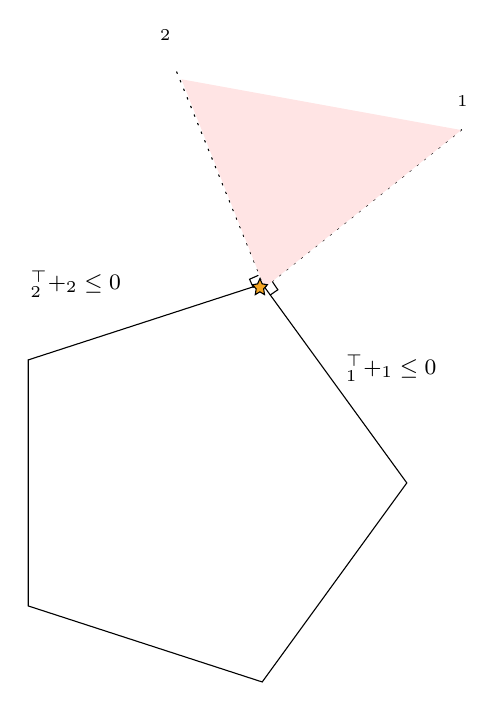
\begin{tikzpicture}[x=0.75pt,y=0.75pt,yscale=-1,xscale=1]
    % Feasible region
    \draw
        (253.95,280.32) -- (184.28,376.22) -- (71.55,339.59)
        -- (71.55,221.06) -- (184.28,184.43) -- cycle;

    % Normal directions and their span
    \draw[dash pattern={on 0.84pt off 2.51pt}]
        (143.01,82.13) -- (170.45,149.39) -- (185.44,186.15);
    \draw[dash pattern={on 0.84pt off 2.51pt}]
        (185.44,186.15) -- (281.41,109.33);
    \draw[draw opacity=0,fill={rgb,255:red,255;green,228;blue,228},fill opacity=1]
        (145.36,85.84) -- (280.19,110.32) -- (185.44,186.15) -- cycle;

    % Right-angle markers
    \draw (189.29,183.53) -- (191.83,187.27) -- (187.98,189.88);
    \draw (180.03,186.32) -- (178.19,182.19) -- (182.44,180.3);

    % Reference point
    \draw[fill={rgb,255:red,245;green,166;blue,35},fill opacity=1]
        (183.17,181.9) -- (184.28,184.43) -- (186.77,184.84)
        -- (184.97,186.81) -- (185.39,189.59) -- (183.17,188.27)
        -- (180.94,189.59) -- (181.37,186.81) -- (179.57,184.84)
        -- (182.06,184.43) -- cycle;

    % Labels
    \node[anchor=north west,inner sep=0.75pt,font=\footnotesize]
        at (223.4,217.52) {$\vg_{1}^{\top}\vy+\evh_{1}\leq 0$};
    \node[anchor=north west,inner sep=0.75pt,font=\footnotesize]
        at (71.4,176.72) {$\vg_{2}^{\top}\vy+\evh_{2}\leq 0$};
    \node[anchor=north west,inner sep=0.75pt,font=\footnotesize]
        at (277,92.72) {$\vg_{1}$};
    \node[anchor=north west,inner sep=0.75pt,font=\footnotesize]
        at (133.8,60.72) {$\vg_{2}$};
\end{tikzpicture}
\end{document}
